\section{Introduction}

\subsection{Classification}
With the rapid growth of computer technology and the emerging online information, classication job has become a crucial techique for the classification of various and massive data. Normally, classification algorithms are used to distinguish between two or more types of data,for example, to determine whether an email is a spam. 

There are multiple approaches that is commonly used for classification: Logistic Regression, K Nearest Neighbor, Decision Tree, Naive Bayes and Support Vector Machine. Though the differrent means of classification may vary, the key processes are mostly the same as illustrated in Figure \ref{fig:The key process of classfication}.

\begin{figure}[h!]
    \centering
    
\includegraphics[width=\textwidth]{figures/The key process of classfication.png}
    \caption{The key process of classification}
    \label{fig:The key process of classfication}
\end{figure}


The classification is the automatic processing and interpretation of patterns/features through the computer using mathematical methods. It contains two parts: feature selection/extraction and data classification. However, the diversity and complexity of the original data bring much difficulty to the classification, especially for the case when a large amount of data is implemented.

\subsection{Support Vector Machine (SVM)}
The Support Vector Machine(SVM) was formally proposed by Vapnik at the 1995 Computer Learning Theory Conference. With 25 years of development, it has become a classic classification method. The theoretical basis of the method  is the principle of VC dimension and structural risk minimization. It overcomes the local minima and dimensional disasters, thus has a great advantage for solving practical problems such as nonlinearity, small samples, high dimensionality and local minimum points\cite{xuegong2000introduction}.


In simple terms, SVM achieves classification by finding a hyperplane of given data. The hyperplane may be in the space where the data is located or mapped to a higher dimensional space by the kernel function. The division of the hyperplane may be strict (hard) or not so strict (soft).


While learning from large-scale samples, SVM still has some deficiencies which manifested in excessive memory consumption, slow training speed and low accuracy\cite{platt1999fast}.


\subsection{Multiclass Problems}
SVM solves two-class problems, that is, it divides the given data into two classes. If we want to apply SVM in multiclass problems, two strategies can be conducted: one-vs-rest strategy and one-vs-one strategy.

\subsubsection{One-vs-Rest Strategy}
One-vs-rest strategy means that each time, consider one of the K classes and the rest of the K classes as two elements of a two-class problem. It divides the K-class problem into K two-class problems. For each two-class problem, a SVM is trained. The final result depends on the discriminant functions of each SVM. For a given data x as input, y is the output value of the discriminant function. And x belongs to the class whose discriminant function has the largest y.

\subsubsection{One-vs-One Strategy}
One-vs-one strategy means that considering any two classes in the multiclass problem as two classes in a two-class problem. Therefore, the K-class problem is divided into K(K-1)/2 two-class problems. For each two-class problem, a SVM is trained.  When a data x is given, each SVM will predict a class in which x belongs to. Generally, voting strategy is used to determine which class x belongs to.

\subsection{Min-Max-Module Strategy}
In order to solve large-scale multiclass problems efficiently  and effortlessly, Lv and Ito(1999) proposed a Min-Max-Modular(\( M^3 \)) network. The subsequent research has verified its validity.

For multiclass problem, a module selection procedure for combination of binary classifiers is proposed for a general combination procedure under the one-vs-one task decomposition strategy\cite{赵海2005最小最大模块化分类器研究}.


Generally, the overview of the Min-Max-Module is shown in Figure \ref{fig:An overview of the Min-Max-Module strategy}\cite{lu2000emergence}. More details will be discussed in the next section.
\begin{figure}[!ht]
    \centering
    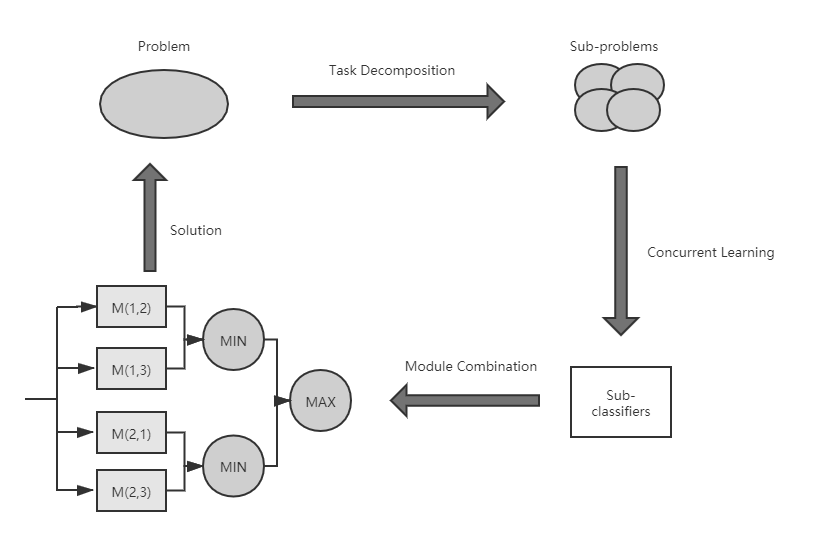
\includegraphics[width=\textwidth]{figures/An overview of the Min-Max-Module strategy.png}
    \caption{An overview of the Min-Max-Module strategy}
    \label{fig:An overview of the Min-Max-Module strategy}
\end{figure}

